%\documentclass[german,10pt]{book}      
\usepackage{makeidx}
\usepackage{babel}            % Sprachunterstuetzung
\usepackage{amsmath}          % AMS "Grundpaket"
\usepackage{amssymb,amsfonts,amsthm,amscd} 
\usepackage{mathrsfs}
\usepackage{rotating}
\usepackage{sidecap}
\usepackage{graphicx}
\usepackage{color}
\usepackage{fancybox}
\usepackage{tikz}
\usetikzlibrary{arrows,snakes,backgrounds}
\usepackage{hyperref}
\hypersetup{colorlinks=true,
                    linkcolor=blue,
                    filecolor=magenta,
                    urlcolor=cyan,
                    pdftitle={Overleaf Example},
                    pdfpagemode=FullScreen,}
%\newcommand{\hyperref}[1]{\ref{#1}}
%
\definecolor{Gray}{gray}{0.80}
\DeclareMathSymbol{,}{\mathord}{letters}{"3B}
%
\newcounter{num}
\renewcommand{\thenum}{\arabic{num}}
\newenvironment{anmerkungen}
   {\begin{list}{(\thenum)}{%
   \usecounter{num}%
   \leftmargin0pt
   \itemindent5pt
   \topsep0pt
   \labelwidth0pt}%
   }{\end{list}}
%
\renewcommand{\arraystretch}{1.15}                % in Formeln und Tabellen   
\renewcommand{\baselinestretch}{1.15}                 % 1.15 facher
                                                      % Zeilenabst.
\newcommand{\Anmerkung}[1]{{\begin{footnotesize}#1 \end{footnotesize}}\\[0.2cm]}
\newcommand{\comment}[1]{}
\setlength{\parindent}{0em}           % Nicht einruecken am Anfang der Zeile 

\setlength{\textwidth}{15.4cm}
\setlength{\textheight}{23.0cm}
\setlength{\oddsidemargin}{1.0mm} 
\setlength{\evensidemargin}{-6.5mm}
\setlength{\topmargin}{-10mm} 
\setlength{\headheight}{0mm}
\newcommand{\identity}{{\bf 1}}
%
\newcommand{\vs}{\vspace{0.3cm}}
\newcommand{\noi}{\noindent}
\newcommand{\leer}{}

\newcommand{\engl}[1]{[\textit{#1}]}
\parindent 1.2cm
\sloppy

         \begin{document}  \setcounter{chapter}{4}


\chapter{Das Zwillingsparadoxon}
% Kap 5
\label{chap_Zwilling}

Das Zwillingsparadoxon geh\"ort zu den bekanntesten Gedankenexperimenten der Physik,
wobei dieser Effekt in abgewandelter Form auch
experimentell \"uberpr\"uft bzw.\ beobachtet wurde.\index{Zwillingsparadoxon} 
Die Idee: Eine Person bleibt hier auf der Erde (die wir n\"aherungsweise als Inertialsystem
ansehen), eine zweite, gleich alte Person - daher betrachtet man gerne Zwillinge - macht
mit einem Raumschiff eine ausgedehnte Weltraumreise mit nahezu Lichtgeschwindigkeit.
Nach einiger Zeit treffen die beiden Personen wieder zusammen und es stellt sich heraus,
dass die Person, die auf der Erde geblieben ist, deutlich mehr gealtert ist als die Person, die den
Weltraumflug gemacht hat. 

An dieser Situation sind zwei Dinge paradox: (1) Wie k\"onnen Zwillinge sich in ihrem
Alter um viele Jahre unterscheiden? - hier liefert die Relativit\"atstheorie eine unmittelbare
Erkl\"arung - und (2) Was unterscheidet das Bezugssystem der Person, die auf der Erde
geblieben ist, von dem Bezugssystem der Person, die die Weltraumreise gemacht hat?
Es muss ja einen physikalischen Grund geben, welche der beiden Personen j\"unger
geblieben ist. Bef\"anden sich z.B.\ beide in einem Inertial\-sys\-tem, m\"usste die Physik auch f\"ur
beide Personen dieselbe sein. Mindestens eine der beiden Personen befand sich also nicht in einem 
Inertialsystem; dies ist die Person, welche die Weltraumreise gemacht hat und irgendwann
mindestens einmal beschleunigen musste, um wieder an den Ausgangsort zur\"uckkommen zu k\"onnen. 
Gelegentlich hei\ss t es deshalb, die Beschleunigung sei daf\"ur verantwortlich, dass die
eine Person j\"unger geblieben ist. Diese Aussage - insbesondere die Sprechweise
\glqq daf\"ur verantwortlich sein\grqq\ - ist irref\"uhrend und f\"uhrt zu vielen
Fehlvorstellungen: Die Beschleunigung hat keinen kausalen Einfluss auf den Gang von
Uhren, aber sie unterscheidet ein Nicht-Inertialsystem von einem Inertialsystem.  

In diesem Kapitel kl\"aren wir zun\"achst den Begriff der Eigenzeit und wie man die
Eigenzeit entlang einer Weltlinie berechnen kann.\index{Weltlinie} 
Als Weltlinie bezeichnen wir eine 
Trajektorie $\pmb{x}(t)$ in einer vierdimensionalen Raumzeit
bzw.\ den Graph der Abbildung $t \mapsto \pmb{x}(t)$.  
Anschlie\ss end wird das Zwillingsparadoxon
nochmals genauer beschrieben und er\"ortert. Begriffe wie Koordinatensystem, Bezugssystem,
Inertialsystem sowie auch das Konzept der Einstein-Synchronisation von Uhren werden vorausgesetzt. 
 
\section{Die Eigenzeit entlang einer Weltlinie}

Eines der Grundpostulate der Speziellen Relativit\"atstheorie ist die Aussage, dass die
Lichtgeschwindigkeit f\"ur einen inertialen Beobachter unabh\"angig vom Bewegungszustand
der Lichtquelle immer denselben Wert hat.\index{Spezielle Relativit\"atstheorie!Grundpostulat}
 Seien $A$ und $B$ zwei Ereignisse, die durch\index{Konstanz der Lichtgeschwindigkeit}
einen Lichtstrahl verbunden werden k\"onnen (z.B.\ ($A$) der Moment, in dem ein Lichtstrahl durch eine
Blende tritt und ($B$) der Moment, in dem dieser Lichtstrahl an einem Spiegel reflektiert wird). 
Zwei solche Ereignisse bezeichnet man als \textit{lichtartig}.\index{lichtartig} 
Dann gilt f\"ur jeden inertialen Beobachter:
\begin{equation} 
             \frac{|\Delta \pmb{x}|}{\Delta t}=c   \hspace{1cm} {\rm oder} 
             \hspace{1cm} (\Delta \pmb{x})^2 - c^2 (\Delta t)^2 =0 \, .
\end{equation}
Hierbei sind $\Delta \pmb{x}$ bzw.\ $\Delta t$ der in einem inertialen Bezugssystem gemessene
Abstand (genauer der Differenzvektor, dessen Betrag der Abstand ist) bzw.\ die Zeitdauer 
zwischen den beiden Ereignissen $A$ und $B$. $c$ bezeichnet die
Lichtgeschwindigkeit im Vakuum und ist somit eine universelle Konstante. Aus dieser
Gleichung wird oft gefolgert, dass
\begin{equation} 
\label{eq_Invarianz1}
            (\Delta \pmb{x})^2 - c^2 (\Delta t)^2 = (\Delta \pmb{x}')^2 - c^2 (\Delta t')^2  \, ,
\end{equation}
wobei sich nun $\Delta \pmb{x}$ bzw.\ $\Delta t$ auf die r\"aumliche Differenz und die Zeitdauer 
zwischen zwei beliebigen Ereignissen $A$ und $B$ bezieht, also nicht unbedingt nur lichtartige 
Ereignisse. $\Delta \pmb{x}'$ und $\Delta t'$ bezeichnen den entsprechenden
Differenzvektor bzw.\ die Zeitdauer zwischen denselben Ereignissen 
in einem anderen inertialen Bezugssystem.

Dieser Schluss ist allerdings zu begr\"unden, denn ganz allgemein
kann man nat\"urlich aus der Gleichheit zweier Ausdr\"ucke an der Stelle 0 nicht auf die Gleichheit
allgemein schlie\ss en und was f\"ur lichtartige Ereignisse gilt, muss
nicht unbedingt f\"ur beliebige Ereignisse gelten. Die wesentlichen weiteren Annahmen, die hier
eingehen sind: (1) der \"Ubergang f\"ur r\"aumliche und zeitliche Abst\"ande von einem inertialen
Bezugssystem in ein anderes inertiales Bezugssystem wird durch eine lineare Transformation
beschrieben, und (2) unser Raum ist homogen und 
isotrop.\index{homogen (Raum)}\index{isotrop} 

Die erste Annahme, die Linearit\"at der Transformation, bedeutet, dass sich die linke und die rechte
Seite von Gleichung \ref{eq_Invarianz1} nur um einen Faktor unterscheiden k\"onnen. Die Annahme
begr\"undet sich daraus, dass unter den Transformationen Inertialsysteme wieder in Inertialsysteme
\"ubergehen sollen, sodass in einem Raum-Zeit-Diagramm gerade Linien wieder in gerade
Linien transformiert werden. Aus der Isotropie und Homogenit\"at des Raumes folgt dann, dass dieser
Faktor 1 sein muss.\footnote{Die inverse Transformation muss wegen der Isotropie denselben
Faktor haben wie die Transformation selbst, daher kommt f\"ur den Faktor nur noch $\pm 1$ in Frage.
Da man aber (in mehr als einer Raumdimension) eine Transformation stetig in ihr Inverses
\"uberf\"uhren kann, muss der Faktor $+1$ sein.} 

Seien nun $A$ und $B$ zwei Ereignisse, sodass
das Ereignis $B$ durch das Ereignis $A$ kausal beeinflusst werden kann. Das bedeutet:
\begin{equation} 
\label{eq_kausal}
              c^2 (\Delta t)^2 > (\Delta \pmb{x})^2     \, .
\end{equation}
Gilt diese Eigenschaft f\"ur zwei Ereignisse in einem Inertialsystem, dann gilt sie in allen
Inertialsystemen. Man bezeichnet die Ereignisse $A$ und $B$ in diesem Fall als 
\textit{zeitartig} bzw.\ genauer als \textit{relativ zeitartig zueinander}.\index{zeitartig}
(Die Begriffe lichtartig, zeitartig und raumartig (s.u.) kennzeichnen immer eine Relation
zwischen zwei Ereignissen; f\"ur ein einzelnes Ereignis sind diese Begriffe sinnlos.)
Zu zwei zeitartigen Ereignissen gibt es immer ein Inertialsystem, sodass diese beiden 
Ereignisse am Ort $x=0$ (oder allgemeiner am selben Ort) stattfinden. F\"ur dieses Inertialsystem
ist $\Delta \pmb{x} =0$ und somit wird der Abstand zwischen diesen beiden Ereignissen 
ausschlie\ss lich durch die Zeitdauer $\Delta \tau$ zwischen ihnen in diesem ausgezeichneten
Inertialsystem charakterisiert. Diese spezielle Zeitdauer bezeichnet man als die 
\textit{Eigenzeit}\index{Eigenzeit}
des Streckenabschnitts der inertialen Weltlinie, die die beiden Ereignisse verbindet.

Man beachte, dass die Eigenzeit nicht einfach zwei Ereignissen, sondern einer Weltlinie, die
die Ereignisse verbindet, zugeschrieben wird. Handelt es sich bei dieser Weltlinie um die
Weltlinie des Ursprungs 
eines Inertialsystems, wie oben angenommen, bezeichnet man diese Eigenzeit auch als Abstand der
beiden Ereignisse. Handelt es sich bei den Ereignissen um 
\textit{raumartige} Ereignisse,\index{raumartig}
gilt $c^2 (\Delta t)^2 < (\Delta \pmb{x})^2$. In diesem Fall gibt es immer ein Inertialsystem, in dem
die beiden Ereignisse gleichzeitig stattfinden, d.h.\ in diesem Inertialsystem ist $\Delta t=0$ und
der r\"aumlich Abstand der Ereignisse ist $|\Delta \pmb{x}|$. Man beachte, dass diese
Zuordnungen - Eigenzeiten zu zwei zeitartigen Ereignissen und Abstand zu raumartigen
Ereignissen - ein spezielles Inertialsystem voraussetzen. Andererseits ist beispielsweise die
Eigenzeit zwischen zwei Ereignissen $A$ und $B$ eine Lorentz-Invariante:\index{Lorentz-Invariante} 
Alle Beobachter sind sich darin einig, dass eine (ideale) Uhr, die sich im Ursprung eines 
Inertialsystems befindet und deren Weltlinie die Ereignisse $A$ und $B$ verbindet, 
diese Eigenzeit anzeigt.   

Wir k\"onnen den Begriff der Eigenzeit von einer geraden Strecke in einem Inertialsystem
zu einer beliebigen Weltlinie verallgemeinern. Sei $\pmb{x}(t)$ die Weltlinie eines Beobachters. 
Wir k\"onnen diese Weltlinie in kleine Abschnitte unterteilen, die geradlinig verbunden werden.
Die Weltlinie wird also durch einen Polygonzug angen\"ahert. F\"ur jede infinitesimale
Teilstrecke ist
\begin{equation}
\label{eq_Eigenzeit0}
           (\Delta \tau (t))^2 =  (\Delta t)^2 - \frac{1}{c^2}(\Delta \pmb{x})^2 
           \hspace{1cm} {\rm bzw.} \hspace{1cm}
       \Delta \tau (t) =  \sqrt{ 1  -\frac{1}{c^2} \left( \frac{\Delta \pmb{x}}{\Delta t} \right)^2} ~ \Delta t
\end{equation}
die Eigenzeit. Hierbei sind $\Delta t$ und $\Delta \pmb{x}$ die Zeitdifferenz und
die r\"aumliche Differenz in einem beliebigen Inertialsystem. Im Sinne eines Riemann'schen
Integrals k\"onnen wir schreiben
\begin{equation}
\label{eq_Eigenzeit}
              \tau(\gamma) = \int_\gamma {\rm d}\tau = \int_{t_0}^{t_1} 
               \sqrt{ 1  -\frac{1}{c^2} \left( \frac{{\rm d} \pmb{x}}{{\rm d} t} \right)^2} ~ {\rm d} t \, .
\end{equation}
$\gamma$ ist hierbei eine Weltlinie,\index{Weltlinie} 
die in einem beliebigen Inertialsystem durch
die Zeit $t$ in diesem System parametrisiert und durch $\pmb{x}(t)$ beschrieben wird.
$\tau(\gamma)$ ist die Eigenzeit zwischen den beiden Ereignissen $\pmb{x}(t_0)$ und
$\pmb{x}(t_1)$ entlang der Weltlinie $\gamma$.  

An dieser Stelle wurde eine wesentliche Annahme gemacht: Durch die Beschleunigung
in nicht-inertialen Systemen wird der Gang einer Uhr nicht zus\"atzlich beeinflusst. 
Es tr\"agt nur die Eigenzeit bei, die sich aus einer Summe der geraden (inertialen)
Abschnitte der durch einen Polygonzug angen\"aherten Weltlinie ergibt. Die
\glqq Knicke\grqq\ geben keinen zus\"atzlichen Beitrag. 

Au\ss erdem beachte man, dass die direkte Verbindungsweltlinie zwischen zwei Ereignissen,
also die Verbindung in einem Inertialsystem, die gr\"o\ss te Eigenzeit hat - alle anderen
Weltlinien, die dieselben beiden Ereignisse verbinden, haben k\"urzere Eigenzeiten. 
Dies ist umgekehrt zur euklidischen Geometrie, wo die direkte Verbindung die k\"urzeste
Verbindung ist. Der Unterschied beruht auf dem Minuszeichen in 
Gl.\ \ref{eq_Eigenzeit}: Je schneller ein Weg durchlaufen wird, umso k\"urzer ist die
Eigenzeit; und jeder Weg, der zwei Ereignisse nicht direkt verbindet, muss insgesamt
schneller durchlaufen werden.

\section{Die Euklid- und Minkowski-Schablone}

Wenn wir in der euklidischen Ebene den Abstand von zwei Punkten $A$ und $B$ bestimmen m\"ochten,
legen wir ein Lineal (mit Abstandsmarkierungen) an, sodass die beiden Punkte von dem
Lineal verbunden werden, und bilden die Differenz zwischen den Abstandsmarkierungen
der beiden Punkte. Das bedeutet einerseits, dass wir die L\"ange der k\"urzesten Verbindungsstrecke
zwischen den beiden Punkten - einer Geraden - ausmessen und nicht die L\"ange einer anderen Verbindungslinie,
und andererseits setzen wir voraus, dass die L\"ange eines Lineals nicht davon abh\"angt, an welchem
Punkt und unter welcher Orientierung wir das Lineal anlegen. 

In einem kartesischen Koordinatensystem ist der euklidische Abstand $d(A,B)$ zwischen zwei Punkten 
$A$ und $B$ durch 
\begin{equation}
                   d(A,B) = \sqrt{(\Delta x)^2 + (\Delta y)^2}
\end{equation}
gegeben. Dieses Abstandsma\ss\ ist offensichtlich invariant unter Transformationen,
f\"ur die
\begin{equation}
                  (\Delta x)^2 + (\Delta y)^2  =   (\Delta x')^2 + (\Delta y')^2
\end{equation}
gilt, wobei sich $\Delta x'$ und $\Delta y'$ auf die Koordinatendifferenzen zwischen den beiden
Punkten in einem anderen kartesischen Koordinatensystem beziehen. Dieses andere Koordinatensystem
kann dabei durch eine Verschiebung, Drehung oder Spiegelung aus dem urspr\"unglichen Koordinatensystem
hervorgegangen sein. Und dies sind genau die Transformationen, f\"ur die der Ausdruck
$(\Delta x)^2 + (\Delta y)^2$ eine Invariante ist.  

Wir k\"onnen den Abstand zwischen zwei Punkten in der euklidischen Ebene aber auch anders
bestimmen:\index{Euklid-Schablone} 
Wir betrachten eine Schablone (siehe Abb.\ \ref{fig_Schablone}, links) aus konzentrischen 
Kreisen mit \"aquidistanten Radien. Legen wir den Mittelpunkt dieser Scheibe auf einen Punkt $A$, 
k\"onnen wir die Distanz zu $B$ an dem Radius des Kreises ablesen, auf dem $B$ liegt. Hierbei 
nutzen wir aus, dass die Punkte auf einem Kreis alle denselben Abstand von einem Zentralpunkt
haben (das ist eine m\"ogliche  Definition eines Kreises).  

\begin{figure}[htb]
\mbox{~}~
\begin{tikzpicture}
\draw[thick] (4,3) circle (0.4);
\draw[thick] (4,3) circle (0.8);
\draw[thick] (4,3) circle (1.2);
\draw[thick] (4,3) circle (1.6);
\draw[thick] (4,3) circle (2.0);
\draw[thick] (4,3) circle (2.4);
\draw[thick] (4,3) circle (2.8);
\draw[thick] (4,3) circle (3.2);
\filldraw[fill=black!100] (4,3) circle (0.06);
\filldraw[fill=black!100] (5.2,4.6) circle (0.06);
\draw (4.15,2.95) node{${\scriptstyle A}$};
\draw (5.4,4.65) node{${\scriptstyle B}$};
\draw (3.86,3) node{${\scriptstyle 0}$};
\draw (3.48,3) node{${\scriptstyle 1}$};
\draw (3.08,3) node{${\scriptstyle 2}$};
\draw (2.68,3) node{${\scriptstyle 3}$};
\draw (2.28,3) node{${\scriptstyle 4}$};
\draw (1.88,3) node{${\scriptstyle 5}$};
\draw (1.48,3) node{${\scriptstyle 6}$};
\draw (1.08,3) node{${\scriptstyle 7}$};
\draw (0.68,3) node{${\scriptstyle 8}$};
%\filldraw[fill=black!100] (13,3) circle (0.04);
\end{tikzpicture}
\hspace{1.0cm}
\begin{tikzpicture}
\draw[thick] (0,6) -- (6,0); 
\draw[thick] (0,0) -- (6,6); 
\filldraw[fill=black!100] (3,3) circle (0.06);
\filldraw[fill=black!100] (4.2,4.6) circle (0.06);
\draw (3.19,3) node{${\scriptstyle A}$};
\draw (4,4.65) node{${\scriptstyle B}$};
\draw (2.85,3) node{${\scriptstyle 0}$};
\draw (3,3.53) node{${\scriptstyle 1}$};
\draw (3,3.93) node{${\scriptstyle 2}$};
\draw (3,4.26) node{${\scriptstyle 3}$};
\draw (3,4.64) node{${\scriptstyle 4}$};
\draw (3,5.0) node{${\scriptstyle 5}$};
\draw (3,5.4) node{${\scriptstyle 6}$};
\draw (3,5.8) node{${\scriptstyle 7}$};
%   oben
\draw[thick] (0.05,6) .. controls (2.75,3.4) .. (3,3.4) .. controls (3.25,3.4) ..  (5.95,6); 
\draw[thick] (0.1,6) .. controls (2.5,3.8) .. (3,3.8) .. controls (3.5,3.8) .. (5.9,6); 
\draw[thick] (0.2,6) .. controls (2.9,3.5) and (3.1,3.5) .. (5.8,6); 
\draw[thick] (0.3,6) .. controls (2.7,4.0) and (3.3,4.0) .. (5.7,6); 
\draw[thick] (0.4,6) .. controls (2.6,4.5) and (3.4,4.5) .. (5.6,6); 
\draw[thick] (0.7,6) .. controls (2.5,5.0) and (3.5,5.0) .. (5.3,6); 
\draw[thick] (1,6) .. controls (2.4,5.5) and (3.6,5.5) .. (5,6); 
% unten
\draw[thick] (0.05,0) .. controls (2.75,2.6) .. (3,2.6) .. controls (3.25,2.6) ..  (5.95,0); 
\draw[thick] (0.1,0) .. controls (2.5,2.2) .. (3,2.2) .. controls (3.5,2.2) .. (5.9,0); 
\draw[thick] (0.2,0) .. controls (2.9,2.5) and (3.1,2.5) .. (5.8,0); 
\draw[thick] (0.3,0) .. controls (2.7,2.0) and (3.3,2.0) .. (5.7,0); 
\draw[thick] (0.4,0) .. controls (2.6,1.5) and (3.4,1.5) .. (5.6,0); 
\draw[thick] (0.7,0) .. controls (2.5,1.0) and (3.5,1.0) .. (5.3,0); 
\draw[thick] (1,0) .. controls (2.4,0.5) and (3.6,0.5) .. (5,0); 
%   rechts
\draw[thick] (6,0.05) .. controls (3.4,2.75) .. (3.4,3) .. controls (3.4,3.25) ..  (6,5.95); 
\draw[thick] (6,0.1) .. controls (3.8,2.5) .. (3.8,3) .. controls (3.8,3.5) .. (6,5.9); 
\draw[thick] (6,0.2) .. controls (3.5,2.9) and (3.5,3.1) .. (6,5.8); 
\draw[thick] (6,0.3) .. controls (4,2.7) and (4,3.3) .. (6,5.7); 
\draw[thick] (6,0.4) .. controls (4.5,2.6) and (4.5,3.4) .. (6,5.6); 
\draw[thick] (6,0.7) .. controls (5.0,2.5) and (5.0,3.5) .. (6,5.3); 
\draw[thick] (6,1) .. controls (5.5,2.4) and (5.5,3.6) .. (6,5); 
%   links
\draw[thick] (0,0.05) .. controls (2.6,2.75) .. (2.6,3) .. controls (2.6,3.25) ..  (0,5.95); 
\draw[thick] (0,0.1) .. controls (2.2,2.5) .. (2.2,3) .. controls (2.2,3.5) .. (0,5.9); 
\draw[thick] (0,0.2) .. controls (2.5,2.9) and (2.5,3.1) .. (0,5.8); 
\draw[thick] (0,0.3) .. controls (2.0,2.7) and (2.0,3.3) .. (0,5.7); 
\draw[thick] (0,0.4) .. controls (1.5,2.6) and (1.5,3.4) .. (0,5.6); 
\draw[thick] (0,0.7) .. controls (1.0,2.5) and (1.0,3.5) .. (0,5.3); 
\draw[thick] (0,1) .. controls (0.5,2.4) and (0.5,3.6) .. (0,5); 
\end{tikzpicture}
\caption{\label{fig_Schablone}%
Die Euklid-Schablone (links) und die Minkowski-Schablone (rechts). Die Punkte $A$ und $B$
im euklidischen Raum (links) haben einen Abstand 5: $A$ liegt im Zentrum und $B$ auf dem
Kreis mit der Markierung $5$. Die Punkte $A$ und $B$ auf der rechten Seite haben den
Abstand 3, da $B$ auf der Hyperbel mit der Markierung 3 liegt. In beiden F\"allen bezieht sich
\glqq Abstand\grqq\ immer auf die L\"ange einer geraden Verbindungslinie zwischen beiden Punkten.} 
\end{figure}

In \"ahnlicher Weise k\"onnen wir auch den Abstand zweier Punkte in einem Minkowski-Diagramm
bestimmen.\index{Minkowski-Schablone} 
Hierbei nutzen wir aus, dass $(\Delta t)^2 - (\Delta x)^2$ eine Invariante
ist und die Wurzel aus diesem Ausdruck die L\"ange (Eigenzeit) einer geraden Verbindung
zwischen zwei Punkten ist (vgl.\ Gl.\ \ref{eq_Eigenzeit0}).\footnote{Hier und in den folgenden
Gleichungen verwenden wir Einheiten, in denen $c$ den Wert 1 annimmt.} Dazu verwenden wir
eine Minkowski-Schablone (dies ist ebenso wie Euklid-Schablone kein g\"angiger Fachausdruck sondern 
eine von mir gew\"ahlte Bezeichnung), bei der Hyperbeln die Punkte konstanten Abstands vom Ursprung
anzeigen (siehe Abb.\ \ref{fig_Schablone}, rechts). 

Um den Abstand zwischen zwei Ereignissen in einem Raum-Zeit-Diagramm zu
ermitteln, legen wir die Schablone mit ihrem Zentrum auf eines der Ereignisse und k\"onnen
nun ablesen, auf welcher Hyperbel das andere Ereignis liegt (in Abb.\ \ref{fig_Schablone}, rechts,
hat Ereignis $B$ den Abstand 3 von Ereignis $A$). Man beachte, dass \glqq Abstand\grqq\ wieder
die L\"ange einer geraden Verbindung zwischen den Ereignissen bezeichnet. Das ist bei
zeitartigen Ereignissen die Eigenzeit in dem ausgezeichneten Inertialsystem, in dem die
beiden Ereignisse $A$ und $B$ am selben Raumpunkt stattfinden. Bei raumartigen Ereignissen ist das
der euklidische Abstand in einem Inertialsystem, in dem die Ereignisse gleichzeitig stattfinden.
Lichtartige Ereignisse haben immer den Abstand 0. Da der Lichtkegel f\"ur alle Beobachter derselbe ist,
kann man die Schablone nun nicht in der Raum-Zeit-Ebene drehen.  
Andererseits spielt es keine Rolle, welches Inertialsystem
man als Ursprung w\"ahlt, d.h.\ welches Inertialsystem die senkrechte Zeitachse nach oben auszeichnet.

Wie schon erw\"ahnt, ist die Euklid-Schablone invariant unter Verschiebungen, Spiegelungen und
Drehungen. Entsprechend ist die Minkowski-Schablone invariant unter Verschiebungen, Spiegelungen
an der Zeit- oder Raumachse und unter\index{Lorentz-Transformation} 
Lorentz-Transformationen. (Spezielle) Lorentz-Transformationen 
lassen den Ursprung fest, ebenso die Lichtkegel. Sie transformierten Geraden wieder in Graden
(zeitartige Graden in zeitartige Graden und raumartige in raumartige), sodass jeder Punkt auf seiner
Hyperbel bleibt. 

Diese Konzepte lassen sich auf mehr Raumdimensionen verallgemeinern: Die Euklid-Schablone wird in
drei Dimensionen zu konzentrischen Kugelschalen und die Minkowski-Schablone erh\"alt man, indem 
man die obige Konstruktion in h\"oheren Dimensionen um die Zeitachse dreht. In 2+1 Raum-Zeit-Dimensionen
wird der Lichtkegel zu einem richtigen (Doppel-)Kegelmantel, die zeitartigen Hyperbeln erhalten die
Form von Schalen und die raumartigen Hyperbeln die Form von Reifenfelgen. 

\section{Das Zwillingsparadoxon}

Wir sind nun in der Lage, das Zwillingsparadoxon der speziellen\index{Zwillingsparadoxon}
Relativit\"atstheorie zu erl\"autern. Dazu betrachten wir zwei Personen (Zwillinge),
die unterschiedliche Weltlinien durchlaufen (siehe Abb.\ \ref{fig_Twin}). Person 
A befinde sich in einem Inertialsystem, d.h.\ ihre Weltlinie ist eine Gerade. Diese
Gerade durchlaufe die Ereignisse $A_0$ bis $A_4$. Person B durchlaufe eine
Weltlinie, die sich bei Ereignis $B_0=A_0$ von Person A trennt und sich von A
mit gro\ss er Geschwindigkeit entfernt. Bei $B_2$ bremst die Person B ab und
beschleunigt anschlie\ss end zur\"uck - dies wird in Abb.\ \ref{fig_Twin} als Knick
dargestellt, k\"onnte aber auch durch eine glatte Kurve beschrieben werden. Bei dem Ereignis
$B_4=A_4$ treffen die beiden Personen wieder zusammen.  

\begin{SCfigure}[50][htb]
\begin{picture}(120,170)(-15,0)
\put(50,10){\line(0,1){160}}
\put(50,30){\line(2,3){40}}
\put(90,90){\line(-2,3){40}}
\put(50,30){\makebox(0,0){{\footnotesize $\bullet$}}}
\put(50,150){\makebox(0,0){{\footnotesize $\bullet$}}}
\put(50,90){\makebox(0,0){{\footnotesize $\bullet$}}}
\put(90,90){\makebox(0,0){{\footnotesize $\bullet$}}}
\put(50,75){\makebox(0,0){{\footnotesize $\bullet$}}}
\put(50,105){\makebox(0,0){{\footnotesize $\bullet$}}}
\put(42,30){\makebox(0,0){${\scriptstyle A_0}$}}
\put(42,70){\makebox(0,0){${\scriptstyle A_1}$}}
\put(42,90){\makebox(0,0){${\scriptstyle A_2}$}}
\put(42,110){\makebox(0,0){${\scriptstyle A_3}$}}
\put(42,150){\makebox(0,0){${\scriptstyle A_4}$}}
\put(57,30){\makebox(0,0){${\scriptstyle B_0}$}}
\put(100,90){\makebox(0,0){${\scriptstyle B_2}$}}
\put(57,150){\makebox(0,0){${\scriptstyle B_4}$}}
\qbezier(0,97.5)(50,52.5)(100,97.5)
\qbezier(0,82.3)(50,127.3)(100,82.3)
\end{picture}
\caption{\label{fig_Twin}%
Zum Zwillingsparadoxon: Die Weltlinie
von Zwilling A verl\"auft entlang der
Ereignisse $A_0=B_0$, $A_1$, $A_2$, $A_3$, $A_4=B_4$,
die von Zwilling B entlang $B_0,B_2,B_4$.
Die Weltlinie von Zwilling A ist l\"anger
als die von Zwilling B, d.h., Zwilling A
ist bei der Wiedervereinigung in 
Ereignis $A_4=B_4$ \"alter als sein Zwillingspartner.
Bei $B_2$ hat Zwilling B dasselbe
Alter wie Zwilling A bei $A_1$. Andererseits ist die Eigenzeit zwischen
$A_3$ und $A_4$ dieselbe wie die zwischen $B_2$ und $B_4$.
Insgesamt ist
Zwilling A um die Zeitspanne zwischen $A_1$ und
$A_3$ \"alter.}
\end{SCfigure}

Legen wir nun unsere Minkowski-Schablone in den Punkt $A_0$ so erkennen
wir, dass die Eigenzeit von $A_0$ bis $A_1$ f\"ur Person A genauso lang ist wie
die Eigenzeit von Person B von $B_0(=A_0)$ bis zum Ereignis $B_2$. Diese beiden
Punkte liegen auf einer zeitartigen Hyperbel. Umgekehrt k\"onnen wir unsere
Schablone in den Punkt $A_4$ legen und erkennen, dass die Eigenzeit von Ereignis
$A_3$ bis $A_4$ f\"ur Person A genauso lang ist, wie die Eigenzeit von 
$B_2$ bis $B_4$ f\"ur Person B. F\"ur Person B haben wir aber damit die
gesamte Weltlinie ausgemessen: Sie hat dieselbe L\"ange (Eigenzeit), wie die
beiden Abschnitte der Weltlinie von Person A von $A_0$ bis $A_1$ plus $A_3$ bis
$A_4$. F\"ur Person A kommt aber noch die Eigenzeit von Abschnitt $A_1$ bis $A_3$
hinzu. Um diese Eigenzeit ist Person A beim abschlie\ss enden Zusammentreffen
\"alter als Person B. 

\section{Die Rolle der Beschleunigung}

In seinen ber\"uhmten \glqq Feynman Lectures on Physics\grqq\ beschreibt 
Feynman in\index{Feynman, Richard}
Kapitel 16-2 auch das Zwillingsparadoxon. Er schreibt dort \textit{... the man who has felt
the accelerations ... is the one who would be younger}. Diese (und \"ahnliche Bemerkungen
in anderen Lehrb\"uchern) haben gelegentlich dazu gef\"uhrt, dass die Beschleunigung als Ursache
daf\"ur angesehen wird, dass der eine Zwilling j\"unger bleibt. Andererseits haben wir oben
betont, dass die Beschleunigung keinen Einfluss auf den Gang einer (idealen) Uhr haben soll
und die L\"ange einer Weltlinie nicht davon abh\"angt, wie viele Beschleunigungsphasen
auftreten, sondern nur davon, wie lang die Summe der infinitesimalen inertialen Abschnitte
ist, durch die wir die Weltlinie immer besser ann\"ahern k\"onnen (also das Riemann'sche
Integral in Gl.\ \ref{eq_Eigenzeit}; in das nur die Geschwindigkeit aber keine
Beschleunigung eingeht). 

Tats\"achlich ist auch die Beschleunigung nicht die Ursache daf\"ur, dass eine Person
j\"unger geblieben ist, aber das behauptet Feynman auch nicht. Die Beschleunigungsphase
ist lediglich die physikalisch nachweisbare Eigenschaft, um die sich das Bezugs\-sys\-tem von B von dem 
Bezugssystem von A unterscheidet (damit ist gemeint, dass man in einem lokalen,
abgeschlossenen Labor feststellen kann, dass eine Beschleunigung vorliegt). W\"aren die beiden Bezugssysteme
physikalisch gleichwertig (w\"urde es sich beispielsweise bei beiden Bezugssystemen um 
Inertialsysteme handeln), w\"urde aus dem Relativit\"atsprinzip folgen, dass auch die Physik in
beiden Systemen die gleiche sein muss und damit kann nicht in dem einen System mehr und dem anderen
weniger Eigenzeit vergangen sein. Die Tatsache, dass die Beschleunigungsphase die beiden
Bezugs\-sys\-teme unterscheidet, bedeutet nicht, dass die Beschleunigung auch die unmittelbare
Ursache daf\"ur ist, dass diese Person j\"unger geblieben ist.

\begin{SCfigure}[50][htb]
\begin{picture}(120,170)(0,0)
\put(50,10){\line(0,1){160}}
\put(50,30){\line(2,3){40}}
\put(90,90){\line(-2,3){40}}
\put(50,75){\line(2,3){10}}
\put(60,90){\line(-2,3){10}}
\put(50,30){\makebox(0,0){{\footnotesize $\bullet$}}}
\put(50,150){\makebox(0,0){{\footnotesize $\bullet$}}}
\put(50,90){\makebox(0,0){{\footnotesize $\bullet$}}}
\put(90,90){\makebox(0,0){{\footnotesize $\bullet$}}}
\put(50,75){\makebox(0,0){{\footnotesize $\bullet$}}}
\put(50,105){\makebox(0,0){{\footnotesize $\bullet$}}}
\put(60,90){\makebox(0,0){{\footnotesize $\bullet$}}}
\put(42,30){\makebox(0,0){${\scriptstyle A_0}$}}
\put(42,70){\makebox(0,0){${\scriptstyle A_1}$}}
\put(42,90){\makebox(0,0){${\scriptstyle A_2}$}}
\put(42,110){\makebox(0,0){${\scriptstyle A_3}$}}
\put(42,150){\makebox(0,0){${\scriptstyle A_4}$}}
\put(57,30){\makebox(0,0){${\scriptstyle B_0}$}}
\put(100,90){\makebox(0,0){${\scriptstyle B_2}$}}
\put(57,150){\makebox(0,0){${\scriptstyle B_4}$}}
\put(67,90){\makebox(0,0){${\scriptstyle C_2}$}}
%\qbezier(0,97.5)(50,52.5)(100,97.5)
%\qbezier(0,82.3)(50,127.3)(100,82.3)
\end{picture}
\caption{\label{fig_Drill}%
Erweiterung des Zwillingsparadoxons f\"ur
Drillinge. Die drei Weltlinien -- ($A_0 \rightarrow
A_1 \rightarrow A_2 \rightarrow A_3 \rightarrow A_4$)
f\"ur Drilling A, ($A_0 \rightarrow A_1 \rightarrow 
C_2 \rightarrow A_3 \rightarrow A_4$) f\"ur
Drilling C und ($B_0 \rightarrow B_2 \rightarrow B_4$)
f\"ur Drilling B -- sind unterschiedlich
lang. Insbesondere ist die Weltlinie von 
Drilling B  k\"urzer als die von Drilling C, obwohl
beide dieselben Beschleunigungsphasen
erlebt haben.}
\end{SCfigure}

Um dieses Argument zu untermauern, betrachten wir in Abb.\ \ref{fig_Drill} eine etwas erweiterte 
Situation. Nun sind drei Personen (Drillinge) gleichen Alters gegeben: A, B und C. Die Personen A und B
durchlaufen dieselben Weltlinien wie oben. Die Person C verbleibt jedoch bei Person A
bis zum Ereignis $A_1$. W\"ahrend A weiterhin in einem Inertialsystem verbleibt, beschleunigt
C von A weg bis zum Ereignis $C_2$, kehrt dort um und trifft bei $A_3$ wieder mit A zusammen. 
Wir haben es nun also mit drei Weltlinien zu tun. Wie man in Abb.\ \ref{fig_Drill} erkennen kann,
sind die Beschleunigungsphasen von B und C identisch: Eine Beschleunigung von A weg
(bei $B_0$ und $A_1$) eine Beschleunigung f\"ur die Wende (bei $C_2$ und $B_2$) und ein
Abbremsen in das Inertialsystem von A (bei $A_3$ und $B_4$). Die Beschleunigungen sind auch
gleich gro\ss. Doch obwohl Person C dieselben Beschleunigungsphasen mitgemacht hat
wie B, ist die Weltlinie von B deutlich k\"urzer und Person B ist am Ende die J\"ungste. 
Person C ist \"alter als B (trotz derselben Beschleunigungphasen) aber j\"unger als A. 
Der wichtige Unterschied in den Bezugs\-sys\-temen von C und B besteht nicht in den Beschleunigungsphasen,
sondern in den Zeitdauern zwischen den Beschleunigungsphasen bzw.\ den in diesen Zeitdauern
zur\"uckgelegten unterschiedlichen Weltlinien.

Betrachten wir dazu noch ein Beispiel aus der euklidischen Geometrie (siehe Abb.\ \ref{fig_Dreieck}). 
Dort gilt die Dreiecksungleichung:\index{Dreiecksungleichung} 
$d(A,C) \leq d(A,B) + d(B,C)$. Feynmans Bemerkung k\"onnte 
man auf diesen Fall \"ubertragen: Der Weg von $A$ nach $C$, der einen Knick hat, ist der l\"angere. 
Oder, wenn wir es physikalischer formulieren wollen: Der Weg von $A$ nach $C$, bei dem
man irgendwann beschleunigen muss, ist der l\"angere. 
Diese Aussage ist sicherlich richtig. Aber es w\"are irref\"uhrend zu sagen, der Knick sei die
Ursache daf\"ur, dass der Weg \"uber den Punkt $B$ der l\"angere sei.   

\begin{SCfigure}[50][htb]
\begin{picture}(120,90)(0,0)
\put(10,10){\line(1,0){100}}
\put(10,10){\line(2,3){40}}
\put(110,10){\line(-1,1){60}}
\put(10,10){\makebox(0,0){{\footnotesize $\bullet$}}}
\put(110,10){\makebox(0,0){{\footnotesize $\bullet$}}}
\put(50,70){\makebox(0,0){{\footnotesize $\bullet$}}}
\put(5,5){\makebox(0,0){${\scriptstyle A}$}}
\put(55,75){\makebox(0,0){${\scriptstyle B}$}}
\put(115,5){\makebox(0,0){${\scriptstyle C}$}}
\end{picture}
\caption{\label{fig_Dreieck}%
Ein Dreieck in der Euklidischen Ebene. Der Weg von Punkt
$A$ nach Punkt $C$ \"uber den Punkt $B$ ist l\"anger als der direkte
Weg. Trotzdem w\"urde man den Knick bei $B$ nicht als Ursache daf\"ur ansehen,
dass dieser Weg l\"anger ist, obwohl jeder Weg, der l\"anger als die direkte (gerade)
Verbindungslinie ist, einen Knick (oder Bogen) haben muss.}
\end{SCfigure}

Damit erhebt sich die Frage, welche Rolle die Beschleunigung f\"ur das unterschiedliche Alter
der Zwillinge denn nun wirklich spielt. Man k\"onnte das Argument von Feynman ja auch
 folgenderma\ss en formulieren: In allen Inertialsystemen ist nach dem Relativit\"atsprinzip 
 die Physik dieselbe, und da es sich bei den Abschnitten $B_0$ nach $B_2$ einerseits und
 $B_2$ nach $B_4$ andererseits um inertiale Weltlinien handelt, ebenso wie f\"ur Beobachter
 A die gesamte Weltlinie von $A_0$ bis $A_4$, kann der Unterschied in den beiden Weltlinien
 nur von dem \glqq Knick\grqq\ bei $B_2$, also der Beschleunigungsphase, herr\"uhren. 

Vielleicht sollte man hier einen Unterschied machen zwischen \glqq Ursache f\"ur etwas sein\grqq\ 
und \glqq Indiz f\"ur etwas sein\grqq. Nach den Postulaten der Relativit\"atstheorie
gibt es keine gesonderten 
Beitr\"age zur Eigenzeit, wenn ein Sys\-tem beschleunigt wird. Uhren laufen in solchen Phasen 
bzw.\ Momenten nicht 
pl\"otzlich schneller oder langsamer oder machen Spr\"unge. Aber eine Beschleunigungsphase zu haben
ist eine notwendige und hinreichende Bedingung daf\"ur, dass ein Bezugssystem kein Inertial\-sys\-tem
ist, und damit gilt f\"ur ein solches System auch das Relativit\"atsprinzip nicht mehr. Unter den 
unendlich vielen Weltlinien, die zwei zeitartige Ereignisse miteinander verbinden, gibt es nur eine,
die den Ursprung eines Inertialsystem definiert, und diese Weltlinie hat keine Beschleunigungsphase.
Alle anderen Weltlinien haben eine k\"urzere Eigenzeit und notwendigerweise eine Beschleunigungsphase.
Allerdings h\"angt die Eigenzeit einer Weltlinie nicht davon ab, wie viele Beschleunigungsphasen 
auftreten oder wie gro\ss\ die Beschleunigungen sind. Die folgenden Beispiele sollen dies
noch einmal verdeutlichen. 

\begin{figure}[htb]
%   Bild 1
\begin{picture}(140,200)(0,0)
\thicklines
\put(30,0){\line(0,1){200}}
\put(30,10){\line(1,2){45}}
\put(30,190){\line(1,-2){45}}
\put(30,50){\line(3,4){37.3}}
\put(30,150){\line(3,-4){37.3}}
\put(30,10){\makebox(0,0){{\footnotesize $\bullet$}}}
\put(30,50){\makebox(0,0){{\footnotesize $\bullet$}}}
\put(30,190){\makebox(0,0){{\footnotesize $\bullet$}}}
\put(30,150){\makebox(0,0){{\footnotesize $\bullet$}}}
\put(67,100){\makebox(0,0){{\footnotesize $\bullet$}}}
\put(75,100){\makebox(0,0){{\footnotesize $\bullet$}}}
\put(30,100){\makebox(0,0){{\footnotesize $\bullet$}}}
\put(22,10){\makebox(0,0){${\scriptstyle A_0}$}}
\put(22,50){\makebox(0,0){${\scriptstyle A_1}$}}
\put(22,100){\makebox(0,0){${\scriptstyle A_2}$}}
\put(22,150){\makebox(0,0){${\scriptstyle A_3}$}}
\put(22,190){\makebox(0,0){${\scriptstyle A_4}$}}
\put(37,10){\makebox(0,0){${\scriptstyle B_0}$}}
\put(83,100){\makebox(0,0){${\scriptstyle B_2}$}}
\put(37,190){\makebox(0,0){${\scriptstyle B_4}$}}
\put(58,100){\makebox(0,0){${\scriptstyle C_2}$}}
\put(38,50){\makebox(0,0){${\scriptstyle C_1}$}}
\put(38,150){\makebox(0,0){${\scriptstyle C_3}$}}
\put(60,195){\makebox(0,0){(a)}}
\end{picture}
%   Bild 2
\begin{picture}(160,200)(0,0)
\thicklines
\put(30,0){\line(0,1){200}}
\put(30,10){\line(2,3){60}}
\put(30,190){\line(2,-3){60}}
\put(30,70){\line(2,-3){20}}
\put(30,70){\line(2,3){20}}
\put(30,130){\line(2,-3){20}}
\put(30,130){\line(2,3){20}}

\put(30,10){\makebox(0,0){{\footnotesize $\bullet$}}}
\put(30,70){\makebox(0,0){{\footnotesize $\bullet$}}}
\put(30,130){\makebox(0,0){{\footnotesize $\bullet$}}}
\put(50,40){\makebox(0,0){{\footnotesize $\bullet$}}}
\put(50,160){\makebox(0,0){{\footnotesize $\bullet$}}}
\put(30,190){\makebox(0,0){{\footnotesize $\bullet$}}}
\put(50,100){\makebox(0,0){{\footnotesize $\bullet$}}}
\put(90,100){\makebox(0,0){{\footnotesize $\bullet$}}}
\put(30,100){\makebox(0,0){{\footnotesize $\bullet$}}}
\put(22,10){\makebox(0,0){${\scriptstyle A_0}$}}
\put(22,70){\makebox(0,0){${\scriptstyle A_1}$}}
\put(22,100){\makebox(0,0){${\scriptstyle A_2}$}}
\put(22,130){\makebox(0,0){${\scriptstyle A_3}$}}
\put(22,190){\makebox(0,0){${\scriptstyle A_4}$}}
\put(37,10){\makebox(0,0){${\scriptstyle B_0}$}}
\put(96,100){\makebox(0,0){${\scriptstyle B_2}$}}
\put(37,190){\makebox(0,0){${\scriptstyle B_4}$}}
\put(58,100){\makebox(0,0){${\scriptstyle C_2}$}}
\put(58,40){\makebox(0,0){${\scriptstyle C_1}$}}
\put(58,160){\makebox(0,0){${\scriptstyle C_3}$}}
\put(60,195){\makebox(0,0){(b)}}
\end{picture}
%   Bild 3
\begin{picture}(120,200)(0,0)
\thicklines
\put(30,0){\line(0,1){200}}
\put(0,0){\line(2,3){100}}
\put(0,200){\line(2,-3){100}}
\put(30,45){\makebox(0,0){{\footnotesize $\bullet$}}}
\put(67,100){\makebox(0,0){{\footnotesize $\bullet$}}}
\put(30,155){\makebox(0,0){{\footnotesize $\bullet$}}}
\put(23,45){\makebox(0,0){${\scriptstyle A}$}}
\put(23,155){\makebox(0,0){${\scriptstyle C}$}}
\put(74,100){\makebox(0,0){${\scriptstyle B}$}}
\put(60,195){\makebox(0,0){(c)}}
\put(37,8){\makebox(0,0){A}}
\put(0,11){\makebox(0,0){B}}
\put(107,55){\makebox(0,0){C}}
\end{picture}
\caption{\label{fig_TwinAcc}%
Verschiedene Beschleunigungsphasen im Zwillings- bzw.\ Drillingsparadoxon.
(a) Eine Abwandlung des Drillingsparadoxons: Person C hat st\"arkere Beschleunigungsphasen
als Person B. Durch geeignete Verschiebung der Abst\"ande - ohne Ver\"anderung der
Beschleunigungen - kann man erreichen, dass die Weltlinie von C l\"anger oder
k\"urzer ist als die von B. (b) Person C beschleunigt nun mehrfach und bewegt sich
entlang einer Zickzacklinie, wohingegen Person B nur einmal
beschleunigt (in Ereignis $B_2$). Trotzdem sind B und C beim Wiedersehen in
Ereignis $A_4$ gleich alt. (c) Die drei Intertialsysteme (A, B, C) treffen sich paarweise
in den Ereignissen $A$, $B$ und $C$ und synchronisieren in diesen Momenten
ihre Uhren. Es finden keine Beschleunigungen statt.  
In $C$ treffen A und C zusammen und vergleichen ihre Uhren. Die Uhr von A zeigt
mehr verflossene Zeit an als die Uhr von C. }
\end{figure}

In Abbildung \ref{fig_TwinAcc} sind verschiedene Abwandlung des Zwillingsparadoxons dargestellt.
In Abb.\ \ref{fig_TwinAcc} (a) ist nochmals das Drillingsparadoxon aus Abb.\ \ref{fig_Drill} wiedergegeben,
allerdings hat Person B nun vergleichsweise schwache Beschleunigungsphasen wohingegen
Person C st\"arkeren Beschleunigungen unterliegt. Allein durch Variation der Abst\"ande zwischen den
Ereignissen (z.B.\ den Ereignissen $A_1$ und $A_3$, bei denen Person C zur Weltreise ansetzt)
kann man erreichen, dass entweder die Weltlinie von C k\"urzer ist als die von B oder aber l\"anger. 
Die Weltlinie von Person A, die keine Beschleunigungen erf\"ahrt, bleibt nat\"urlich die l\"angste.
Dieses Beispiel zeigt, dass die St\"arke der Beschleunigungen nicht dar\"uber entscheidet, welche
Weltlinie l\"anger und welche k\"urzer ist. 

In Abb.\ \ref{fig_TwinAcc} (b) hat Person C mehrere Beschleunigungsphasen, die der
Beschleunigung von Person B im Punkt $B_2$ entsprechen. Person C fliegt k\"urzere Strecken
im Zickzack und beschleunigt bei $C_1$, $A_1$, $C_2$, $A_3$ und $C_3$ (abgesehen von
den Beschleunigungsphasen bei $B_0$ und $B_4$, die Person C mit Person B gemeinsam hat). 
Trotzdem sind die Weltlinien von C und B gleich lang. Das zeigt, dass die Anzahl der
Beschleunigungsphasen nicht dar\"uber entscheidet, welche Weltlinie k\"urzer oder l\"anger ist. 

Schlie\ss lich haben wir es in Abb.\ \ref{fig_TwinAcc} (c) mit drei intertialen Weltlinien A, B und C
zu tun. Hier finden \"uberhaupt keine Beschleunigungen statt, allerdings werden bei den 
Ereignissen $A$ und $B$ Uhren synchronisiert. Bei Ereignis $A$ synchronisierten Person A und
B ihre Uhren, bei Ereignis $B$ synchronisieren nochmals Person B und C ihre Uhren und zwar
derart, dass C seine Uhr auf die Uhr von B einstellt. 

Es werden also verschiedene Uhren entlang
der Weltlinie von $A$ \"uber $B$ nach $C$ so synchronisiert, dass die jeweilige Uhr die
Eigenzeit entlang dieser Weltlinie anzeigt. Andererseits zeigt die Uhr von Person A die Eigenzeit
der Weltlinie A an. Wenn sich bei $C$ die Personen A und C mit ihren Uhren treffen, zeigt 
die Uhr von C weniger Zeit an als die Uhr von A und zwar in demselben Ma\ss, in dem ein
Zwilling entlang der Weltlinie \"uber $B$ j\"unger geblieben w\"are. 

Dieses letzte Beispiel ist gleichzeitig ein Beweis, dass bei einer Beschleunigung keine
zus\"atzliche Beeinflussung einer Uhr und damit der Eigenzeit entlang einer Weltlinie stattfindet. 
Die Uhren selbst werden nicht beschleunigt, sondern lediglich an den Treffpunkten, wo auch
keine Laufzeitverz\"ogerungen der Signal\"ubertragung ber\"ucksichtigt werden m\"ussen, synchronosiert. 
Die Uhr von Person C, die letztendlich bei Ereignis $C$ wieder mit A zusammentrifft, zeigt
dieselbe Zeit an, die auch eine Uhr angezeigt h\"atte, die bei den Ereignissen $A$ und $B$
beschleunigt worden w\"are. 
 
\section{Vergleich der Bezugssysteme}

Nachdem wir in den vergangenen Abschnitten festgestellt haben, dass die Beschleunigung
keinen unmittelbaren Einfluss auf den Gang einer Uhr hat und somit nicht die Ursache
f\"ur die unterschiedlichen Eigenzeiten entlang der verschiedenen Weltlinien ist, kommen wir
nochmals auf die Frage zur\"uck, welche Rolle die Beschleunigung bei dem Zwillingsparadoxon
spielt. Insbesondere interessiert in diesem Zusammenhang, was der Zwilling in einem
Bezugssystem von den Ereignissen auf der Weltlinie des Zwillings in dem jeweils anderen 
Bezugssystem beobachtet. Es zeigt sich, dass die Beschleunigung in diesem Fall eine sehr 
gro\ss e Rolle spielt. 

\begin{figure}[htb]
\begin{picture}(200,150)(-40,0)
\thicklines
\put(50,10){\line(0,1){130}}
\put(50,30){\line(2,3){60}}
\put(110,10){\line(0,1){130}}
\put(18,30){\line(2,3){33}}
\thinlines
\put(19,59){\line(3,2){101}}
\put(20,120){\line(1,0){110}}
\put(50,30){\makebox(0,0){{\footnotesize $\bullet$}}}
\put(50,100){\makebox(0,0){{\footnotesize $\bullet$}}}
\put(50,120){\makebox(0,0){{\footnotesize $\bullet$}}}
\put(110,120){\makebox(0,0){{\footnotesize $\bullet$}}}
\put(50,79.5){\makebox(0,0){{\footnotesize $\bullet$}}}
\put(42,30){\makebox(0,0){${\scriptstyle A_0}$}}
\put(42,82){\makebox(0,0){${\scriptstyle A_1}$}}
\put(44,105){\makebox(0,0){${\scriptstyle A_2}$}}
\put(44,115){\makebox(0,0){${\scriptstyle A_3}$}}
\put(50,5){\makebox(0,0){\small A}}
\put(110,5){\makebox(0,0){\small A1}}
\put(80,63){\makebox(0,0){\small B}}
\put(10,30){\makebox(0,0){\small B1}}
\put(57,30){\makebox(0,0){${\scriptstyle B_0}$}}
\put(117,115){\makebox(0,0){${\scriptstyle B_2}$}}
%\put(57,150){\makebox(0,0){${\scriptstyle B_4}$}}
\qbezier(-10,120)(50,81)(110,120)
%\qbezier(0,82.3)(50,127.3)(100,82.3)
\end{picture}
\hspace{1cm}
%
\begin{picture}(150,150)(0,0)
\thicklines
\put(50,10){\line(0,1){130}}
\put(50,120){\line(2,-3){60}}
\put(110,10){\line(0,1){130}}
\thinlines
\put(40,77){\line(3,-2){80}}
\put(20,30){\line(1,0){110}}
\put(50,120){\makebox(0,0){{\footnotesize $\bullet$}}}
\put(50,50){\makebox(0,0){{\footnotesize $\bullet$}}}
\put(50,30){\makebox(0,0){{\footnotesize $\bullet$}}}
\put(110,30){\makebox(0,0){{\footnotesize $\bullet$}}}
\put(50,70.5){\makebox(0,0){{\footnotesize $\bullet$}}}
\put(42,120){\makebox(0,0){${\scriptstyle A_6}$}}
\put(42,68){\makebox(0,0){${\scriptstyle A_5}$}}
\put(44,45){\makebox(0,0){${\scriptstyle A_4}$}}
\put(44,35){\makebox(0,0){${\scriptstyle A_3}$}}
\put(50,5){\makebox(0,0){\small A}}
\put(110,5){\makebox(0,0){\small A1}}
\put(80,87){\makebox(0,0){\small B}}
\put(57,120){\makebox(0,0){${\scriptstyle B_4}$}}
\put(117,35){\makebox(0,0){${\scriptstyle B_2}$}}
%\put(57,150){\makebox(0,0){${\scriptstyle B_4}$}}
\qbezier(-10,30)(50,69)(110,30)
%\qbezier(0,82.3)(50,127.3)(100,82.3)
\end{picture}
\caption{\label{fig_Twin2}%
Die verschiedenen Phasen des Zwillingsparadoxons. (links)
Der erste Teil der Reise von Zwilling B bis kurz vor dem Umkehrpunkt $B_2$. (rechts) Der
zweite Teil der Reise nach dem Umkehrpunkt $B_2$. (Erl\"auterungen siehe Text.)}
\end{figure}

Betrachten wir zun\"achst den ersten Teil der Reise, bis Zwilling B das Ereignis
$B_2$ erreicht. In Abb.\ \ref{fig_Twin2}, links, sind die Weltlinien von vier Beobachtern
dargestellt: (A) die Weltlinie von Zwilling A, (A1) eine zweite Weltlinie in dem 
Bezugssystem von A (also parallel zur Weltlinie von A), allerdings geht diese Weltlinie
durch das Ereignis $B_2$; (B) die Weltlinie von B und (B1) die Weltlinie eines
zweiten Beobachters in dem Bezugssystem von B. Au\ss erdem ist eine waagerechte
Linie durch die Ereignisse $A_3$ und $B_2$ dargestellt: Sie repr\"asentiert alle
Ereignisse, die in dem Bezugssystem von A zum selben Zeitpunkt wie das Ereignis
$B_2$ stattfinden. Eine weitere Gleichzeitigkeitslinie durch die Punkte $A_1$ und $B_2$
repr\"asentiert alle Ereignisse, die im Bezugssystem von B gleichzeitig zum Ereignis
$B_2$ sind. 

Man erkennt nun Folgendes: Rein objektiv, ohne auf die unterschiedlichen globalen 
Gleichzeitigkeitsdefinitionen von A
und B Bezug zu nehmen, zeigen die Uhren von A und B in den Ereignissen $A_2$ und $B_2$     
dieselbe Zeit an - sie liegen auf derselben Hyperbel der Minkowski-Schablone. 
Wenn jedoch Zwilling B das Ereignis $B_2$ erreicht, hat Zwilling 
A bez\"uglich seiner Gleichzeitigkeitsdefinition das Ereignis $A_3$ erreicht. Auf der Uhr von A
ist aber bei diesem Ereignis mehr Zeit vergangen, als auf der Uhr von B. Daher hat A den
Eindruck, die Uhr von B gehe langsamer (entsprechend der bekannten Zeitdilatation in der
Speziellen Relativit\"atstheorie). Dies wird allerdings nicht direkt von A gemessen, sondern
in seinem Bezugssystem von A1, dessen Uhren mit A synchronisiert sind.
F\"ur den Beobachter B bzw.\ in seinem Bezugssystem hat
A aber erst das Ereignis $A_1$ erreicht, wenn B bei $B_2$ ankommt. Von dem Beobachter
B1, der sich im Bezugssystem von B befindet und dessen Uhr mit der von B synchronisiert
ist, wird registriert, dass bei diesem Ereignis auf der Uhr von A weniger Zeit vergangen ist.
Insofern hat man in dem Bezugssystem von B den Eindruck, die Uhren in dem System A
gingen langsamer.  

Abb.\ \ref{fig_Twin2}, rechts, zeigt die gleiche Situation f\"ur den zweiten Teil der Reise,
nachdem Beobachter B bei $B_2$ beschleunigt hat und sich nun wieder auf A zubewegt. 
Die Ereignisse $A_3$ und $B_2$ sind f\"ur A gleichzeitig (wie vorher), nun sind f\"ur B aber
die Ereignisse $A_5$ und $B_2$ gleichzeitig. Die Eigenzeit, angezeigt von der Uhr von B,
zwischen den Ereignissen $B_2$ und $A_6=B_4$, ist dieselbe, wie die Eigenzeit in dem
System von A zwischen den Ereignissen $A_4$ und $A_6$. Insgesamt kommen wir wieder
zu dem Ergebnis, dass die Gesamtzeit, die im Bezugssystem von B vergangen ist, gleich
den beiden Zeitdauern $A_0$ bis $A_2$ plus $A_4$ bis $A_6$ im Bezugssystem von A ist,
und in diesem Bezugssystem die Zeitdifferenz zwischen $A_2$ und $A_4$ zus\"atzlich vergangen ist.

Wir erkennen jetzt die besondere Bedeutung der Beschleunigung in $B_2$: Sie ver\"andert
in diesem \glqq Moment\grqq\ die Gleichzeitigkeitslinien von Bezugssystem B und zwar derart,
dass kurz vor dem Ereignis $B_2$ f\"ur Beobachter $B$ das Ereignis $A_1$ gleichzeitig ist,
und unmittelbar nach dem Ereignis $B_2$ ist es das Ereignis $A_5$. Durch die Beschleunigung verpasst
Beobachter B also alle Ereignisse zwischen $A_1$ und $A_5$ (bzw., da jede Beschleunigung
eine endliche Zeitdauer ben\"otig, werden diese Ereignisse in dem Bezugssystem von $B$
in einem beliebig kurzen Zeitraum
\glqq erlebt\grqq). Man k\"onnte etwas \"ubertrieben sagen, dass f\"ur Zwilling $B$ die Ereignisse zwischen 
$A_2$ und $A_4$ im Bezugssystem von A  aufgrund der \glqq unendlichen\grqq\
Beschleunigung keine Zeitzuordnung haben. 

In diesem Zusammenhang ist anzumerken, dass die Konstruktion von globalen Gleichzeitigkeitslinien
(bzw.\ in drei Raumdimensionen \glqq Gleichzeitigkeitsr\"aumen\grqq) eine Besonderheit der
Speziellen Relativit\"atstheorie ist. Diese Konstruktion ist nur sinnvoll, solange man es mit
Inertialsystemen zu tun hat, deren Weltlinien Geraden sind. Rein operational setzt sie voraus,
dass sich zwei Beobachter im selben Bezugssystem f\"ur die Zeit, w\"ahrend der sie im
Sinne der Einstein-Synchronisation\index{Einstein-Synchronisation} 
ihre Signale austauschen, auf geraden Weltlinien bewegen. 
Sobald ein Bezugssystem eine Beschleunigung erf\"ahrt, machen solche globalen Gleichzeitigkeitslinien
keinen Sinn mehr: In manchen Bereichen l\"auft die Zeit r\"uckw\"arts, in anderen l\"auft sie
beliebig schnell vorw\"arts; und operational l\"asst sich eine Einstein-Synchronisation in diesen
F\"allen nicht sinnvoll durchf\"uhren (sie w\"urde verschiedene Gleichzeitigkeitsdefinitionen
f\"ur Beobachter im selben Bezugs\-sys\-tem ergeben). Daher betrachtet man in der Allgemeinen
Relativit\"atstheorie auch lieber das, was ein Beobachter von den Ereignissen wirklich sieht, d.h.,
man ber\"ucksichtigkeit die Laufzeitverz\"ogerungen durch die endliche Ausbreitungsgeschwindigkeit
von Licht. In der Speziellen Relativit\"atstheorie sollte man dies bei beschleunigten Bezugssystemen
ebenfalls tun. 
 
\section{Kuriosit\"aten}
 
\subsection{Das Zwillingsparadoxon in einem periodischen Universum}

In einem r\"aumlich periodischen Universum\index{Zwillingsparadoxon!in periodischem Universum} 
k\"onnen zwei verschiedene inertiale Weltlinien 
dieselben zwei Ereignisse verbinden. Ein solches periodisches Universum kann lokal dem
flachen Minkowski-Raum entsprechen und ist somit eine L\"osung der Einstein-Gleichungen
der allgemeinen Relativit\"atstheorie. Die Einstein-Gleichungen legen keine globalen
topologischen Eigenschaften der Raum-Zeit fest.

Wir betrachten wieder zwei Bezugssysteme (Beobachter)
A und B. Bezugs\-sys\-tem A ist \glqq in Ruhe\grqq\ und die zugeh\"orige Weltline verbindet
die beiden Ereignisse $A$ und $B$ direkt. Bezugssystem B hat bez\"uglich A eine bestimmte Geschwindigkeit.
Die beiden Bezugssysteme treffen sich bei Ereignis $A$. Bezugssystem B bewegt sich nun mit
seiner Geschwindigkeit weiter, windet sich einmal um das periodische Universum und trifft bei
Ereignis $B$ wieder mit Bezugssystem A zusammen (siehe Abb.\ \ref{fig_Periodic}). 

\begin{SCfigure}[50][htb]
\begin{picture}(105,150)(0,0)
\put(10,15){\line(0,1){120}}
\put(90,15){\line(0,1){120}}
\qbezier(30,10)(-10,15)(30,20)
\qbezier(70,10)(110,15)(70,20)
\qbezier(30,20)(50,22)(70,20)
\qbezier(30,10)(50,8)(70,10)
\qbezier(30,130)(-10,135)(30,140)
\qbezier(70,130)(110,135)(70,140)
\qbezier(30,140)(50,142)(70,140)
\qbezier(30,130)(50,128)(70,130)
\qbezier(50,75)(90,64)(90,57)
\qbezier(10,93)(10,86)(50,75)
\thicklines
\put(50,0){\line(0,1){150}}
\qbezier(50,40)(10,33)(10,23)
\qbezier(50,40)(90,47)(90,57)
\qbezier(50,110)(10,103)(10,93)
\qbezier(50,110)(90,117)(90,127)
\put(50,40){\makebox(0,0){{\footnotesize $\bullet$}}}
\put(50,110){\makebox(0,0){{\footnotesize $\bullet$}}}
\put(56,36){\makebox(0,0){${\scriptstyle A}$}}
\put(56,105){\makebox(0,0){${\scriptstyle B}$}}
\put(57,0){\makebox(0,0){A}}
\put(20,40){\makebox(0,0){B}}
\end{picture}
\caption{\label{fig_Periodic}%
Das Zwillingsparadoxon in einem r\"aumlich periodischen Universum.
Eine Persion bleibt an ihrem Ort, die andere bewegt sich mit konstanter
Geschwindigkeit einmal um \glqq das Universum\grqq\ herum. Beide
trennen sich bei Ereignis $A$, wo sie gleich alt sind bzw.\ ihre Uhren
sychronisiert haben,  und
treffen bei Ereignis $B$ wieder aufeinander. Person B ist j\"unger als Person A. 
Beide befinden sich w\"ahrend der gesamten Zeit in einem Inertialsystem. 
In diesem Fall gilt jedoch das Relativit\"atsprinzip nicht.}
\end{SCfigure}

Legen wir nun wieder unsere Minkowski-Schablone an die Weltlinien, stellen wir
fest, dass die Weltlinie zwischen den beiden Ereignissen $A$ und $B$ von Bezugssystem B 
k\"urzer ist als die Weltlinie von A. Doch in diesem Fall sind beide Bezugssysteme
Inertialsysteme. Wie kann das sein?

Die Antwort auf diesen scheinbaren Widerspruch lautet: Das Relativit\"atsprinzip gilt
nicht mehr.\index{Relativit\"atsprinzip} 
Wir haben oben schon davon gesprochen, dass sich das Bezugssystem
A \glqq in Ruhe\grqq\ befinde. Dieser Ausdruck ist in diesem Fall sinnvoll:
Es gibt nur ein Bezugssystem, f\"ur das die Einstein-Synchronisation von Uhren
global konsistent ist. Das bedeutet Folgendes: Wir k\"onnen in einem r\"aumlich
periodischen Universum die Synchronisation von Uhren an verschiedenen Punkten 
in einem Bezugssystem auf zwei Weisen durchf\"uhren. Wir k\"onnen die beiden Punkte
wegen der Periodizit\"at des Raums auf verschiedene Weisen verbinden (einmal links um
den Torus und einmal rechts um den Torus in Abb.\ \ref{fig_Periodic}) und die Einstein-Synchronisation
entlang beider Richtungen durchf\"uhren. Es gibt nur ein System - und dies bezeichnen wir als
das Ruhesystem - bei dem diese beiden Synchronisationsvorschriften dieselbe Gleichzeitigkeitszuordnung
liefern. Wenn aber ein absolutes Ruhesystem ausgezeichnet und physikalisch
bestimmbar ist, gilt die Lorentz-Invarianz und damit auch das Relativit\"atsprinzip nicht mehr. 

%\end{document}

